\documentclass[12pt]{hedsemwork}
\usepackage[utf8]{inputenc}
\usepackage[T2A]{fontenc}
\usepackage[russian]{babel}
\usepackage{pscyr}
\usepackage{graphicx}
\usepackage[vectors,derivative]{hedmaths}
\usepackage{float}
\renewcommand{\arraystretch}{2}
\renewcommand{\frac}{\dfrac}
\DeclareMathSizes{12}{10}{6}{6}


\faculty{Факультет электроники и вычислительной техники}
\department{<<Физика>>}
\subject{Электродинамика СВЧ}
\student[m]{студент группы Ф-469\\Абдрахманов~В.~Л.}
\teacher[m]{доцент, к.ф.-м.н.\\Грецов~М.~В.}

\begin{document}
\maketitle
\section{Волны в волноводе со слоистым заполнением}
\begin{figure}[h]
    \center
    \includegraphics{scheme}
    \caption{Поперечное сечение волновода}
\end{figure}
\subsection{Быстрые волны}
    Рассмотрим быстрые волны, распространяющиеся в двух частях волновода.
    Запишем уравнения:
    \[
        \left\{
        \begin{array}{l}
            \Delta_\perp E_{1z} + g_1^2 E_{1z} = 0,\\
            \Delta_\perp H_{1z} + g_1^2 H_{1z} = 0,\\
            \Delta_\perp E_{2z} + g_2^2 E_{2z} = 0,\\
            \Delta_\perp H_{2z} + g_2^2 H_{2z} = 0
        \end{array}
        \right.
    \]
    Общее решение имеет вид:
    \[
        \left\{
        \begin{array}{l}
            E_{1z} =
            (A^e_1\cos u^e_1 x + B^e_1\sin u^e_1 x)
            (C^e_1\cos v^e_1 y + D^e_1\sin v^e_1 y)
            e^{i(\omega t - h_1 z)}, \\
            H_{1z} =
            (A^m_1\cos u^m_1 x + B^m_1\sin u^m_1 x)
            (C^m_1\cos v^m_1 y + D^m_1\sin v^m_1 y)
            e^{i(\omega t - h_1 z)}, \\
            E_{2z} =
            (A^e_2\cos u^e_2 x + B^e_2\sin u^e_2 x)
            (C^e_2\cos v^e_2 y + D^e_2\sin v^e_2 y)
            e^{i(\omega t - h_2 z)}, \\
            H_{2z} =
            (A^m_2\cos u^m_2 x + B^m_2\sin u^m_2 x)
            (C^m_2\cos v^m_2 y + D^m_2\sin v^m_2 y)
            e^{i(\omega t - h_2 z)}.
        \end{array}
        \right.
    \]
\subsubsection{Граничные условия}
Теперь воспользуемся граничными условиями и несколько упростим задачу.
На контуре волновода касательная составляющая электрического поля равна нулю,
поэтому
    \[
        E_{1z} = E_1\sin u^e_1 (x-a) \sin \frac{\pi n_1}{b}y
        e^{i(\omega t - h_1 z)},\quad
        E_{2z} = E_2\sin u^e_2 x \sin \frac{\pi n_2}{b}y
        e^{i(\omega t - h_2 z)}.
    \]
Также, учтём, что на границе раздела касательная компонента поля \( \vec{E} \)
непрерывна:
    \[
        E_1\sin u^e_1 (c-a) \sin \frac{\pi n_1}{b}y
        e^{i(\omega t - h_1 z)} =
        E_2\sin u^e_2 c \sin \frac{\pi n_2}{b}y
        e^{i(\omega t - h_2 z)}.
    \]
Равенство должно выполняться при любых \( y \) и \( z \), поэтому
\[
    \boxed{h_1 = h_2 = h,\ n_1 = n_2 = n.}
\]
Для определения вида \( H_{1z} \) найдём \( E_{1x} \):
\begin{align*}
    & E_{1x} =
    -\frac{i}{g_1^2}\left( h\pder{E_{1z}}{x} + \omega\mu\pder{H_{1z}}{y} \right)
    = -\frac{ie^{i(\omega t - h z)}}{g_1^2}\times\\
    &\times\left( h E_1 u^e_1 \cos u^e_1(x-a)\sin\frac{\pi n}{b}y +
    \omega\mu(A^m_1\cos u^m_1 x + B^m_1\sin u^m_1 x)
    (-C^m_1 v^m_1 \sin v^m_1 y + D^m_1 v^m_1 \cos v^m_1 y)\right).
\end{align*}
Так как \( \left.E_{1x}\right|_{y=0,b} = 0 \), то \( D^m_1 = 0 \),
\( v^m_1 = \frac{\pi m_1}{b} y \). Аналогичный результат получается и в области
2:
\[
    \left\{
    \begin{array}{l}
        H_{1z} =
        (A^m_1\cos u^m_1 x + B^m_1\sin u^m_1 x)\cos\frac{\pi m_1}{b}y
        e^{i(\omega t - h z)}, \\
        H_{2z} =
        (A^m_2\cos u^m_2 x + B^m_2\sin u^m_2 x)\cos\frac{\pi m_2}{b}y
        e^{i(\omega t - h z)}.
    \end{array}
    \right.
\]

Теперь воспользуемся компонентами \( E_{1y} \) и \( E_{2y} \):
\begin{align*}
    & E_{1y} = -\frac{i}{g_1^2}\left( h\pder{E_{1z}}{y} -
    \omega\mu\pder{H_{1z}}{x} \right) = \\
    & = -\frac{ie^{i(\omega t - hz)}}{g_1^2}\left( h E_1 \frac{\pi n}{b}
    \sin u^e_1(x-a)\cos\frac{\pi n}{b}y - \omega\mu
    u^m_1 (-A^m_1 \sin u^m_1 x + B^m_1\cos u^m_1 x)\cos\frac{\pi m_1}{b}y
   \right)
\end{align*}
В силу условия \( \left.E_{1y}\right|_{x=a} = 0 \)
\( -A^m_1 \sin u^m_1 x + B^m_1\cos u^m_1 x = H_1\sin u^m_1(x-a) \).
Аналогично, во второй области имеем \(B^m_2=0, A^m_2 = H_2\).
В силу непрерывности на границе раздела \( E_y \), имеем \( m_1 = m_2 = n \).

Выпишем полученные выражения для компонент полей:
\[
    \left\{
    \begin{array}{l}
        E_{1z} = E_1\sin u^e_1 (x-a) \sin \frac{\pi n}{b}y
        e^{i(\omega t - h z)},\\
        H_{1z} = H_1\cos u^m_1 (x-a) \cos \frac{\pi n}{b}y
        e^{i(\omega t - h z)},\\
        E_{2z} = E_2\sin u^e_2 x \sin \frac{\pi n}{b}y
        e^{i(\omega t - h z)},\\
        H_{2z} = H_2\cos u^m_2 x \cos \frac{\pi n}{b}y
        e^{i(\omega t - h z)}.
    \end{array}
    \right.
\]

Отсюда,
\[
    u^e_i = u^m_i = u_i = \sqrt{g_i^2 - \frac{\pi^2n^2}{b^2}}.
\]
\[
    \left\{
    \begin{array}{l}
        E_{1z} = E_1\sin u_1 (x-a) \sin \frac{\pi n}{b}y
        e^{i(\omega t - h z)},\\
        H_{1z} = H_1\cos u_1 (x-a) \cos \frac{\pi n}{b}y
        e^{i(\omega t - h z)},\\
        E_{2z} = E_2\sin u_2 x \sin \frac{\pi n}{b}y
        e^{i(\omega t - h z)},\\
        H_{2z} = H_2\cos u_2 x \cos \frac{\pi n}{b}y
        e^{i(\omega t - h z)}.
    \end{array}
    \right.
\]
Определим также поперечные компоненты:
\[
    \left\{
    \begin{array}{l}
        E_{1x} = -\frac{i e^{i(\omega t - h z)}}{g_1^2}
        \left(h u_1 E_1 - \omega\mu_1\frac{\pi n}{b}H_1\right)
        \cos u_1 (x-a) \sin \frac{\pi n}{b}y,\\
        H_{1x} = \frac{i e^{i(\omega t - h z)}}{g_1^2}
        \left(\omega\eps_1\frac{\pi n}{b}E_1+h u_1 H_1\right)
        \sin u_1 (x-a) \cos \frac{\pi n}{b}y,\\
        E_{1y} = -\frac{i e^{i(\omega t - h z)}}{g_1^2}
        \left(h \frac{\pi n}{b} E_1 + \omega\mu_1u_1H_1\right)
        \sin u_1 (x-a) \cos \frac{\pi n}{b}y,\\
        H_{1y} = -\frac{i e^{i(\omega t - h z)}}{g_1^2}
        \left(\omega\eps_1u_1E_1-h \frac{\pi n}{b} H_1\right)
        \cos u_1 (x-a) \sin \frac{\pi n}{b}y,\\
        E_{2x} = -\frac{i e^{i(\omega t - h z)}}{g_2^2}
        \left(h u_2 E_2 - \omega\mu_2\frac{\pi n}{b}H_2\right)
        \cos u_2 x \sin \frac{\pi n}{b}y,\\
        H_{2x} = \frac{i e^{i(\omega t - h z)}}{g_2^2}
        \left(\omega\eps_2\frac{\pi n}{b}E_2+h u_2 H_2\right)
        \sin u_2 x \cos \frac{\pi n}{b}y,\\
        E_{2y} = -\frac{i e^{i(\omega t - h z)}}{g_2^2}
        \left(h \frac{\pi n}{b} E_2 + \omega\mu_2u_2H_2\right)
        \sin u_2 x \cos \frac{\pi n}{b}y,\\
        H_{2y} = -\frac{i e^{i(\omega t - h z)}}{g_2^2}
        \left(\omega\eps_2u_2E_2-h \frac{\pi n}{b} H_2\right)
        \cos u_2 x \sin \frac{\pi n}{b}y.
    \end{array}
    \right.
\]

Запишем теперь условия непрерывности компонент при \( x = c \):
\begin{equation}
\begin{array}{cl}
    E_{y1} = E_{y2}: &
    \frac{1}{g_1^2} \left(h \frac{\pi n}{b} E_1 + \omega\mu_1u_1H_1\right)
    \sin u_1 (c-a) =  \frac{1}{g_2^2}
    \left(h \frac{\pi n}{b} E_2 + \omega\mu_2u_2H_2\right)
    \sin u_2 c ;\\
    E_{z1} = E_{z2}: & E_1\sin u_1 (c-a) = E_2\sin u_2 c; \\
    H_{y1} = H_{y2}: &
    \frac{1}{g_1^2}\left(\omega\eps_1u_1E_1-h \frac{\pi n}{b} H_1\right)
    \cos u_1 (c-a) = \frac{1}{g_2^2}
    \left(\omega\eps_2u_2E_2-h \frac{\pi n}{b} H_2\right)\cos u_2 c ;\\
    H_{z1} = H_{z2}: & H_1\cos u_1 (c-a) = H_2\cos u_2 c.\\
\end{array}
    \label{eq:fast_waves_continuity}
\end{equation}

\subsubsection{Дисперсионное уравнение}
Выразим амплитуды во второй области через амплитуды в первой из четных уравнений
системы и подставим в нечётные:
\begin{equation}
\begin{array}{l}
    \frac{1}{g_1^2} \left(h \frac{\pi n}{b} E_1 + \omega\mu_1u_1H_1\right)
    \sin u_1 (c-a) =  \frac{1}{g_2^2}
    \left(h \frac{\pi n}{b} E_1 \sin u_1(c-a) +
    \omega\mu_2u_2H_1\cos u_1 (c-a) \tg u_2 c \right) ;\\
    \frac{1}{g_1^2}\left(\omega\eps_1u_1E_1-h \frac{\pi n}{b} H_1\right)
    \cos u_1 (c-a) = \frac{1}{g_2^2}
    \left(\omega\eps_2u_2E_1\sin u_1(c-a)\ctg u_2 c-
    h \frac{\pi n}{b} H_1\cos u_1 (c-a)\right) ;\\
\end{array}
    \label{eq:fast_waves_relations}
\end{equation}
перегруппируем
\[
\begin{array}{l}
    E_1\left(\frac{1}{g_1^2} h \frac{\pi n}{b}\sin u_1 (c-a) -
    \frac{1}{g_2^2}h \frac{\pi n}{b}\sin u_1(c-a)\right) =
    H_1\left(\frac{1}{g_2^2}\omega\mu_2u_2\cos u_1 (c-a) \tg u_2 c-
    \frac{1}{g_1^2}\omega\mu_1u_1\sin u_1 (c-a)\right);\\
    E_1\left(\frac{1}{g_1^2}\omega\eps_1u_1\cos u_1 (c-a)-
    \frac{1}{g_2^2}\omega\eps_2u_2\sin u_1(c-a)\ctg u_2 c\right)=
    H_1\left(\frac{1}{g_1^2}h \frac{\pi n}{b} \cos u_1 (c-a)-
    \frac{1}{g_2^2}h \frac{\pi n}{b} \cos u_1 (c-a)\right)
\end{array}
\]
Отсюда
\begin{align*}
    &\left(\frac{1}{g_1^2} h \frac{\pi n}{b}\sin u_1 (c-a) -
    \frac{1}{g_2^2}h \frac{\pi n}{b}\sin u_1(c-a)\right)\left(\frac{1}{g_1^2}h \frac{\pi n}{b} \cos u_1 (c-a)-
    \frac{1}{g_2^2}h \frac{\pi n}{b} \cos u_1 (c-a)\right) =\\
    & \left(\frac{1}{g_2^2}\omega\mu_2u_2\cos u_1 (c-a) \tg u_2 c-
    \frac{1}{g_1^2}\omega\mu_1u_1\sin u_1 (c-a)\right)
    \left(\frac{1}{g_1^2}\omega\eps_1u_1\cos u_1 (c-a)-
    \frac{1}{g_2^2}\omega\eps_2u_2\sin u_1(c-a)\ctg u_2 c\right).
\end{align*}
\[
    \left( \frac{1}{g_1^2} - \frac{1}{g_2^2} \right)^2\frac{h^2\pi^2n^2}{b^2}=
    \left(\frac{1}{g_2^2}\omega\mu_2u_2\tg u_2 c-
    \frac{1}{g_1^2}\omega\mu_1u_1\tg u_1 (c-a)\right)
    \left(\frac{1}{g_1^2}\omega\eps_1u_1\ctg u_1 (c-a)-
    \frac{1}{g_2^2}\omega\eps_2u_2\ctg u_2 c\right),
\]
\[
    \left( \frac{1}{g_1^2} - \frac{1}{g_2^2} \right)^2\frac{h^2\pi^2n^2}{b^2}=
    \frac{\omega^2u_1u_2}{g_1^2g_2^2}\left(\eps_1\mu_2\frac{\tg u_2 c}{\tg u_1
    (c-a)} + \eps_2\mu_1\frac{\tg u_1 (c-a)}{\tg u_2 c}\right) -\frac{1}{g_1^4}
    \omega^2u_1^2\eps_1\mu_1 - \frac{1}{g_2^4}\omega^2u_2^2\eps_2\mu_2.
\]
Введём обозначение
\[
    A = \frac{\tg u_2 c}{\tg u_1 (c-a)},
\]
с учётом которого уравнение принимает вид
\[
    \frac{2}{g_1^2 g_2^2}\frac{h^2\pi^2n^2}{b^2} =
    -\frac{\omega^2u_1u_2}{g_1^2g_2^2}\left(\eps_1\mu_2 A +
    \eps_2\mu_1\frac{1}{A}\right) +
    \frac{1}{g_1^4}
    \left(\omega^2u_1^2\eps_1\mu_1 + \frac{h^2\pi^2n^2}{b^2}\right) +
    \frac{1}{g_2^4}
    \left(\omega^2u_2^2\eps_2\mu_2 + \frac{h^2\pi^2n^2}{b^2}\right)
\]
Учтём, что
\[
    \omega^2u_i^2\eps_i\mu_i + \frac{h^2\pi^2n^2}{b^2} = \beta_i^2u_i^2 +
    (\beta_i^2 - g_i^2)\frac{\pi^2n^2}{b^2} =
    \beta_i^2\left( u_i^2 + \frac{\pi^2n^2}{b^2} \right) -
    g_i^2\frac{\pi^2n^2}{b^2} =
    g_i^2\left( \beta_i^2 - \frac{\pi^2n^2}{b^2}\right).
\]
Подставив, получим
\[
    \frac{2}{g_1^2 g_2^2}\frac{h^2\pi^2n^2}{b^2} =
    -\frac{\omega^2u_1u_2}{g_1^2g_2^2}\left(\eps_1\mu_2 A +
    \eps_2\mu_1\frac{1}{A}\right) +
    \frac{1}{g_1^2}
    \left(\beta_1^2 - \frac{\pi^2n^2}{b^2}\right) +
    \frac{1}{g_2^2}
    \left(\beta_2^2 - \frac{\pi^2n^2}{b^2}\right)
\]
Домножив на \( g_1^2g_2^2 \), получим:
\[
    2\frac{h^2\pi^2n^2}{b^2} = g_2^2
    \left(\beta_1^2 - \frac{\pi^2n^2}{b^2}\right) +
    g_1^2\left(\beta_2^2 - \frac{\pi^2n^2}{b^2}\right)-
    \omega^2u_1u_2\left(\eps_1\mu_2 A +
    \eps_2\mu_1\frac{1}{A}\right),
\]
Теперь как проще упростить?
\[
    2\frac{h^2\pi^2n^2}{b^2} =
    \beta_1^2 g_2^2 + \beta_2^2 g_1^2 -
    (g_1^2+g_2^2)\frac{\pi^2n^2}{b^2} -
    \omega^2u_1u_2\left(\eps_1\mu_2 A +
    \eps_2\mu_1\frac{1}{A}\right),
\]
\[
    2\frac{h^2\pi^2n^2}{b^2} =
    \beta_1^2 g_2^2 + \beta_2^2 g_1^2 -
    (\beta_1^2+\beta_2^2)\frac{\pi^2n^2}{b^2} +
    2\frac{h^2\pi^2n^2}{b^2} -
    \omega^2u_1u_2\left(\eps_1\mu_2 A +
    \eps_2\mu_1\frac{1}{A}\right),
\]
\[
    \beta_1^2u_2^2 + \beta_2^2u_1^2=
    \omega^2u_1u_2\left(\eps_1\mu_2 A +
    \eps_2\mu_1\frac{1}{A}\right),
\]
Подставляем выражение для \( \beta \) и получаем:
\[
    \eps_1\mu_1\frac{u_2}{u_1} + \eps_2\mu_2\frac{u_1}{u_2} =
    \eps_1\mu_2 A + \eps_2\mu_1\frac{1}{A}
\]
\[
    A^2 - \left(
    \frac{\mu_1}{\mu_2}\frac{u_2}{u_1} + \frac{\eps_2}{\eps_1}\frac{u_1}{u_2}
    \right)A + \frac{\eps_2}{\eps_1}\cdot\frac{\mu_1}{\mu_2} = 0.
\]
По теореме Виета
\[
    A_1 = \frac{\mu_1}{\mu_2}\frac{u_2}{u_1},\quad
    A_2 = \frac{\eps_2}{\eps_1}\frac{u_1}{u_2}.
\]
Таким образом, система имеет решение при выполнении какого-либо из условий
\[
    \frac{\tg u_2 c}{\tg u_1 (c-a)} =
    \frac{\mu_1}{\mu_2}\frac{u_2}{u_1},\quad
    \frac{\tg u_2 c}{\tg u_1 (c-a)} =
    \frac{\eps_2}{\eps_1}\frac{u_1}{u_2}.
\]
Перепишем их в виде
\[
    \left[
        \begin{array}{ll}
            \frac{\mu_1\tg u_1 (a-c)}{u_1} + \frac{\mu_2\tg u_2 c}{u_2} = 0
            \quad & (\mu-\textit{соотношение}),\\
            \frac{u_1\tg u_1 (a-c)}{\eps_1} + \frac{u_2\tg u_2 c}{\eps_2} = 0
            \quad & (\eps-\textit{соотношение}).
        \end{array}
    \right.
\]
Указанные выше выражения получены при условии \( n \neq 0 \). При \( n = 0 \)
имеем \( E_{z1} = E_{z2} = 0 \)
\[
    \left\{
    \begin{array}{l}
        E_{1x} = 0, \\
        H_{1x} = \frac{i e^{i(\omega t - h z)}}{g_1^2}
        h u_1 H_1 \sin u_1 (x-a),\\
        E_{1y} = -\frac{i e^{i(\omega t - h z)}}{g_1^2}
        \omega\mu_1u_1H_1 \sin u_1 (x-a),\\
        H_{1y} = 0,\\
        E_{2x} = 0,\\
        H_{2x} = \frac{i e^{i(\omega t - h z)}}{g_2^2}
        h u_2 H_2 \sin u_2 x,\\
        E_{2y} = -\frac{i e^{i(\omega t - h z)}}{g_2^2}
        \omega\mu_2u_2H_2 \sin u_2 x,\\
        H_{2y} = 0.
    \end{array}
    \right.
\]
Тогда граничные условия записываются в виде:
\[
\begin{array}{cl}
    E_{y1} = E_{y2}: &
    \frac{1}{g_1^2}  \omega\mu_1u_1H_1 \sin u_1 (c-a) =
    \frac{1}{g_2^2}  \omega\mu_2u_2H_2 \sin u_2 c ;\\
    H_{z1} = H_{z2}: & H_1\cos u_1 (c-a) = H_2\cos u_2 c.\\
\end{array}
\]
\[
    \frac{1}{g_1^2} \mu_1 u_1 \tg u_1 (c-a) = \frac{g_2^2} \mu_2 u_2 \tg u_2 c.
\]
При \( n=0 \) \( g_i = u_i \), откуда получаем дисперсионное уравнение
\[
    \frac{\mu_1\tg u_1 (a-c)}{u_1} + \frac{\mu_2\tg u_2 c}{u_2} = 0,
\]
\subsubsection{\(\boldsymbol{\mu}\) - волны}
Теперь используя \( \mu \) - соотношение
\[
    \frac{\mu_1\tg u_1 (a-c)}{u_1} + \frac{\mu_2\tg u_2 c}{u_2} = 0,
\]
определим связь амплитуд продольного электрического и магнитного полей.
Из уравнения первого уравнения системы~(\ref{eq:fast_waves_relations})
\[
    E_1\left(\frac{1}{g_1^2} h \frac{\pi n}{b}-
    \frac{1}{g_2^2}h \frac{\pi n}{b}\right) =
    H_1\left(\frac{1}{g_2^2}\omega\mu_2u_2\frac{\tg u_2 c}{\tg u_1 (c-a)}-
    \frac{1}{g_1^2}\omega\mu_1u_1\right),
\]
\[
    E_1\frac{h\pi n}{b}\left(\frac{1}{g_1^2}-\frac{1}{g_2^2}\right)=
    H_1\left(\frac{1}{g_2^2}\omega\mu_2u_2\frac{\mu_1u_2}{\mu_2u_1}-
    \frac{1}{g_1^2}\omega\mu_1u_1\right),
\]
\[
    E_1 = H_1\frac{\mu_1\omega b}{u_1h\pi n}
    \frac{g_1^2u_2^2 - g_2^2u_1^2}{g_2^2-g_1^2} =
    H_1\frac{\mu_1\omega\pi n}{u_1hb},
\]
Аналогично
\[
    E_2 = H_2{\mu_2\omega\pi n}\frac{u_2hb}.
\]
А из четвёртого уравнения системы~(\ref{eq:fast_waves_continuity}).
\[
    H_2 = H_1\frac{\cos u_1(c-a)}{\cos u_2 c},
\]
Теперь получим выражения для поперечных компонент поля:
\[
    \left\{
    \begin{array}{l}
        E_{1x} = -\frac{i e^{i(\omega t - h z)}}{g_1^2}
            \left(H_1\frac{\mu_1\omega\pi n}{b} -
            \omega\mu_1\frac{\pi n}{b}H_1\right)
            \cos u_1 (x-a) \sin \frac{\pi n}{b}y = 0,\\
        H_{1x} = \frac{i e^{i(\omega t - h z)}}{g_1^2}
            \left(\omega\eps_1\frac{\pi n}{b}H_1\frac{\mu_1\omega\pi n}{u_1hb}+
            h u_1 H_1\right)\sin u_1 (x-a) \cos \frac{\pi n}{b}y =
            i e^{i(\omega t - h z)}\frac{h^2 + \frac{\pi^2 n^2}{b^2}}
            {u_1h}H_1 \sin u_1 (x-a) \cos \frac{\pi n}{b}y,\\
        E_{1y} = -\frac{i e^{i(\omega t - h z)}}{g_1^2}
            \left(h \frac{\pi n}{b} H_1\frac{\mu_1\omega\pi n}{u_1hb} +
            \omega\mu_1u_1H_1\right)
            \sin u_1 (x-a) \cos \frac{\pi n}{b}y = -i e^{i(\omega t - h z)}
            \frac{\mu_1\omega}{u_1} H_1\sin u_1 (x-a) \cos \frac{\pi n}{b}y,\\
        H_{1y} = -\frac{i e^{i(\omega t - h z)}}{g_1^2}
            \left(\omega\eps_1u_1H_1\frac{\mu_1\omega\pi n}{u_1hb}-
            h \frac{\pi n}{b} H_1\right)
            \cos u_1 (x-a) \sin \frac{\pi n}{b}y = -i e^{i(\omega t - h z)}
            \frac{\pi n}{hb}H_1\cos u_1 (x-a) \sin \frac{\pi n}{b}y,\\
        E_{2x} = 0,\\
        H_{2x} = i e^{i(\omega t - h z)}\frac{h^2 + \frac{\pi^2 n^2}{b^2}}
            {u_2h}H_2 \sin u_2 x \cos \frac{\pi n}{b}y,\\
        E_{2y} = -i e^{i(\omega t - h z)}\frac{\mu_2\omega}{u_2} H_2
            \sin u_2 x \cos \frac{\pi n}{b}y,\\
        H_{2y} = -i e^{i(\omega t - h z)}\frac{\pi n}{hb}H_2
            \cos u_2 x \sin \frac{\pi n}{b}y.\\
    \end{array}
    \right.
\]

\subsubsection{\(\boldsymbol{\eps}\) - волны}
А в случае
\[
    \frac{u_1\tg u_1 (a-c)}{\eps_1} + \frac{u_2\tg u_2 c}{\eps_2} = 0,
\]
имеем
\[
    E_1\frac{h\pi n}{b}\left(\frac{1}{g_1^2}-\frac{1}{g_2^2}\right)=
    H_1\left(\frac{1}{g_2^2}\omega\mu_2u_2\frac{u_1\eps_2}{u_2\eps_1}-
    \frac{1}{g_1^2}\omega\mu_1u_1\right),
\]
\[
    H_1 = E_1\frac{\eps_1h\pi n}{u_1\omega b}
    \frac{g_2^2-g_1^2}{g_1^2\eps_2\mu_2 - g_2^2\eps_1\mu_1} =
    -E_1\frac{\eps_1\omega\pi n}{u_1hb},
\]
\[
    E_2 = E_1\frac{\sin u_1(c-a)}{\sin u_2 c},
\]
\[
    H_2 = -E_2\frac{\eps_2\omega\pi n}{u_2hb}.
\]

\[
    \left\{
    \begin{array}{l}
        E_{1x} = -\frac{i e^{i(\omega t - h z)}}{g_1^2}
        \left(h u_1 E_1 +
        \omega\mu_1\frac{\pi n}{b}E_1\frac{\eps_1\omega\pi n}{u_1hb},\right)
        \cos u_1 (x-a) \sin \frac{\pi n}{b}y =-i e^{i(\omega t - h z)}
        \frac{h^2 + \frac{\pi^2 n^2}{b^2}}
        {hu_1}E_1\cos u_1 (x-a) \sin \frac{\pi n}{b}y,\\
        H_{1x} = \frac{i e^{i(\omega t - h z)}}{g_1^2}
        \left(\omega\eps_1\frac{\pi n}{b}E_1-
        h u_1 E_1\frac{\eps_1\omega\pi n}{u_1hb}\right)
        \sin u_1 (x-a) \cos \frac{\pi n}{b}y = 0,\\
        E_{1y} = -\frac{i e^{i(\omega t - h z)}}{g_1^2}
        \left(h \frac{\pi n}{b} E_1 -
        \omega\mu_1u_1E_1\frac{\eps_1\omega\pi n}{u_1hb}\right)
        \sin u_1 (x-a) \cos \frac{\pi n}{b}y = i e^{i(\omega t - h z)}
        \frac{\pi n}{hb} E_1\sin u_1 (x-a) \cos \frac{\pi n}{b}y,\\
        H_{1y} = -\frac{i e^{i(\omega t - h z)}}{g_1^2}
        \left(\omega\eps_1u_1E_1+
        h \frac{\pi n}{b} E_1\frac{\eps_1\omega\pi n}{u_1hb}\right)
        \cos u_1 (x-a) \sin \frac{\pi n}{b}y = -i e^{i(\omega t - h z)}
        \frac{\eps_1\omega}{u_1}E_1\cos u_1 (x-a) \sin \frac{\pi n}{b}y,\\
        E_{2x} = -i e^{i(\omega t - h z)}\frac{h^2 + \frac{\pi^2 n^2}{b^2}}
        {hu_2}E_2\cos u_2 x \sin \frac{\pi n}{b}y,\\
        H_{2x} = 0,\\
        E_{2y} = i e^{i(\omega t - h z)}\frac{\pi n}{hb}
        E_2\sin u_2 x \cos \frac{\pi n}{b}y,\\
        H_{2y} = -i e^{i(\omega t - h z)} \frac{\eps_2\omega}{u_2}
        E_2\cos u_2 x \sin \frac{\pi n}{b}y.\\
    \end{array}
    \right.
\]

\subsection{Поверхностная волна в менее плотной среде}
По условию оптически менее плотной является первая среда. Поэтому рассмотрим
в ней распространение поверхностной волны. Для этого воспользуемся результатами
из предыдущего раздела, заменив в 1 области тригонметрические фугкции аргумента
\(x\) на гиперболические:
\[
    \left\{
    \begin{array}{l}
        E_{1z} = E_1\sh u_1 (x-a) \sin \frac{\pi n}{b}y
        e^{i(\omega t - h z)},\\
        H_{1z} = H_1\ch u_1 (x-a) \cos \frac{\pi n}{b}y
        e^{i(\omega t - h z)},\\
        E_{2z} = E_2\sin u_2 x \sin \frac{\pi n}{b}y
        e^{i(\omega t - h z)},\\
        H_{2z} = H_2\cos u_2 x \cos \frac{\pi n}{b}y
        e^{i(\omega t - h z)}.
    \end{array}
    \right.
\]
Далее, определим соотношение между поперечными волновыми числами:
\[
    \beta_1^2 = h^2 - u_1^2 + \frac{\pi n}{b},
    \beta_2^2 = h^2 + u_2^2 + \frac{\pi n}{b};
\]
\[
    u_1^2 + u_2^2 = \beta_2^2 - \beta_1^2 = \omega^2(\eps_2\mu_2 - \eps_1\mu_1)
\]
Нетрудно заметить, что замена \( u_1 \) на \( iu_1 \) и \( E_1 \) на \( -iE_1 \)
сводит эту задачу к предыдущей. Поэтому воспользуемся теми же дисперсионными
соотношениями, несколько их видоизменив \((\tg iu_1 = i\th u_1)\):
\[
    \left[
        \begin{array}{ll}
            \frac{\mu_1\th u_1 (a-c)}{u_1} + \frac{\mu_2\tg u_2 c}{u_2} = 0
            \quad & (\mu-\textit{соотношение}),\\
            -\frac{u_1\th u_1 (a-c)}{\eps_1} + \frac{u_2\tg u_2 c}{\eps_2} = 0
            \quad & (\eps-\textit{соотношение}).
        \end{array}
    \right.
\]

\subsubsection{\(\boldsymbol{\mu}\) - волны}
\[
    \left\{
    \begin{array}{l}
        E_{1x} = 0,\\
        H_{1x} = i e^{i(\omega t - h z)}\frac{h^2 + \frac{\pi^2 n^2}{b^2}}
            {u_1h}H_1 \sh u_1 x \cos \frac{\pi n}{b}y,\\
        E_{1y} = -i e^{i(\omega t - h z)}\frac{\mu_1\omega}{u_1} H_1
            \sh u_1 x \cos \frac{\pi n}{b}y,\\
        H_{1y} = -i e^{i(\omega t - h z)}\frac{\pi n}{hb}H_1
            \ch u_1 x \sin \frac{\pi n}{b}y.\\
        E_{2x} = 0,\\
        H_{2x} = i e^{i(\omega t - h z)}\frac{h^2 + \frac{\pi^2 n^2}{b^2}}
            {u_2h}H_2 \sin u_2 x \cos \frac{\pi n}{b}y,\\
        E_{2y} = -i e^{i(\omega t - h z)}\frac{\mu_2\omega}{u_2} H_2
            \sin u_2 x \cos \frac{\pi n}{b}y,\\
        H_{2y} = -i e^{i(\omega t - h z)}\frac{\pi n}{hb}H_2
            \cos u_2 x \sin \frac{\pi n}{b}y.\\
    \end{array}
    \right.
\]

\subsubsection{\(\boldsymbol{\eps}\) - волны}
\[
    \left\{
    \begin{array}{l}
        E_{1x} = i e^{i(\omega t - h z)}\frac{h^2 + \frac{\pi^2 n^2}{b^2}}
            {hu_1}E_1\ch u_1 (x-a) \sin \frac{\pi n}{b}y,\\
        H_{1x} = 0,\\
        E_{1y} = i e^{i(\omega t - h z)}\frac{\pi n}{hb}
            E_1\sh u_1 (x-a) \cos \frac{\pi n}{b}y,\\
        H_{1y} = i e^{i(\omega t - h z)}\frac{\eps_1\omega}{u_1}E_1
            \ch u_1 (x-a) \sin \frac{\pi n}{b}y,\\

        E_{2x} = -i e^{i(\omega t - h z)}\frac{h^2 + \frac{\pi^2 n^2}{b^2}}
            {hu_2}E_2\cos u_2 x \sin \frac{\pi n}{b}y,\\
        H_{2x} = 0,\\
        E_{2y} = i e^{i(\omega t - h z)}\frac{\pi n}{hb}
            E_2\sin u_2 x \cos \frac{\pi n}{b}y,\\
        H_{2y} = -i e^{i(\omega t - h z)} \frac{\eps_2\omega}{u_2}
            E_2\cos u_2 x \sin \frac{\pi n}{b}y.\\
    \end{array}
    \right.
\]

\section{Дисперсионные соотношения}
Теперь рассмотрим дисперсионные соотношения. Начнём c LE-волн. Поперечные
волновые числа получаются из решения систем
\[
    \left\{
        \begin{array}{l}
            u_2^2 - u_1^2 = \omega^2(\eps_2\mu_2 - \eps_1\mu_1), \\
            \frac{\mu_1\tg u_1 (a-c)}{u_1} + \frac{\mu_2\tg u_2 c}{u_2}
            = 0
        \end{array}
    \right.
\]
для быстрых волн и
\[
    \left\{
        \begin{array}{l}
            u_2^2 + u_1^2 = \omega^2(\eps_2\mu_2 - \eps_1\mu_1), \\
            \frac{\mu_1\th u_1 (a-c)}{u_1} + \frac{\mu_2\tg u_2 c}{u_2} = 0
        \end{array}
    \right.
\]
для поверхностной волны. Аналитически они не решаются, поэтому представим
результаты численного решения графически. Для отображения обоих классов волн на
одном графике для поверхностной волны будем считать \( u_1^2 < 0 \). Тогда
первые уравнение систем изобразятся прямой, положение которой определяется
частотой, а вторые -- семейством непрерывных кривых. Полученная картина
представлена на рисунке~\ref{fig:le_dispersion}.

\begin{figure}[h]
    \center
    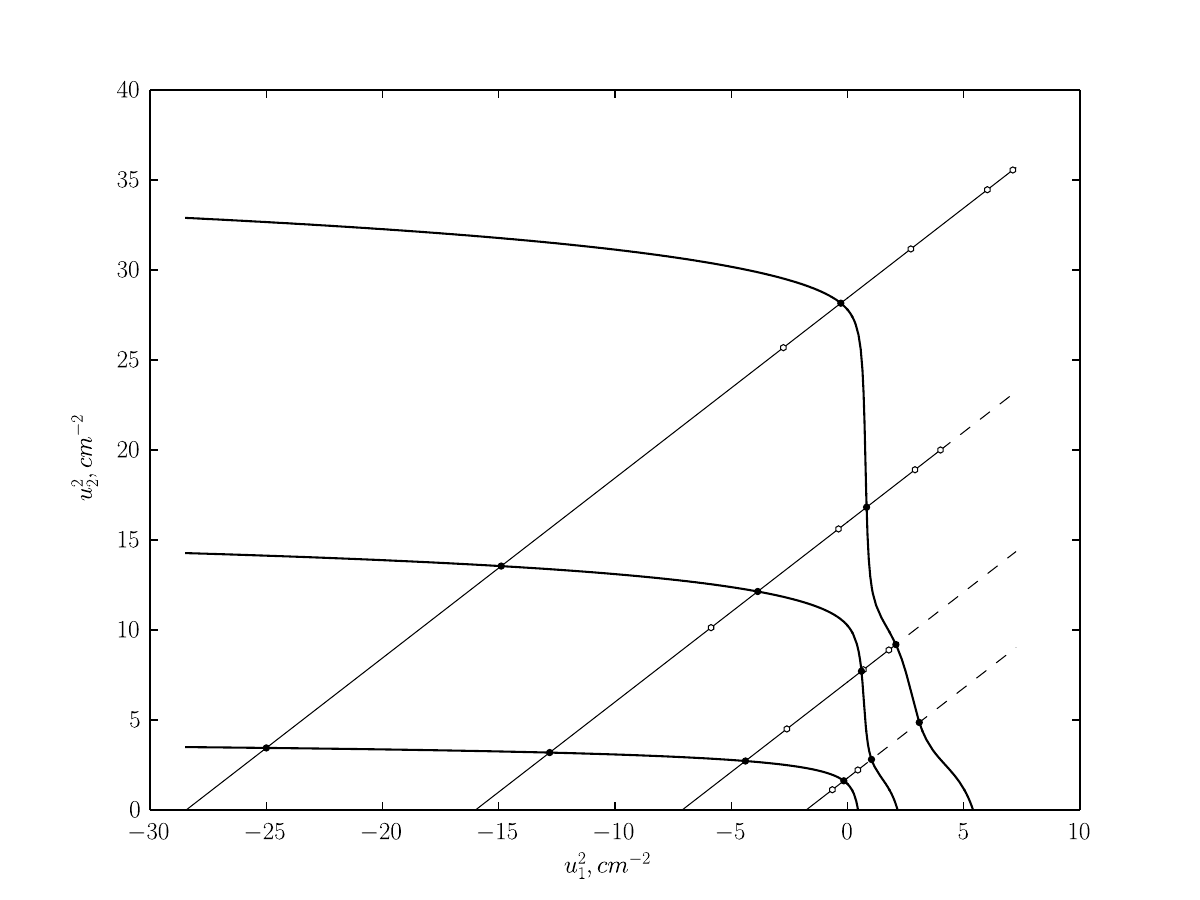
\includegraphics[width=.7\textwidth]{dispersion/le.png}
    \caption{К определению поперечных волновых чисел для LE-волн}
    \label{fig:le_dispersion}
\end{figure}


Совершенно аналогично поступим с LM-волнами. Для них системы имеют вид
\[
    \left\{
        \begin{array}{l}
            u_2^2 - u_1^2 = \omega^2(\eps_2\mu_2 - \eps_1\mu_1), \\
            \frac{u_1\tg u_1 (a-c)}{\eps_1} + \frac{u_2\tg u_2 c}{\eps_2}
            = 0
        \end{array}
    \right.
\]
для быстрых волн и
\[
    \left\{
        \begin{array}{l}
            u_2^2 + u_1^2 = \omega^2(\eps_2\mu_2 - \eps_1\mu_1), \\
            -\frac{u_1\th u_1 (a-c)}{\eps_1} + \frac{u_2\tg u_2 c}{\eps_2} = 0
        \end{array}
    \right.
\]
для поверхностной. Здесь график будет иметь вид, представленный на
рисунке~\ref{fig:lm_dispersion}.

\begin{figure}[h]
    \center
    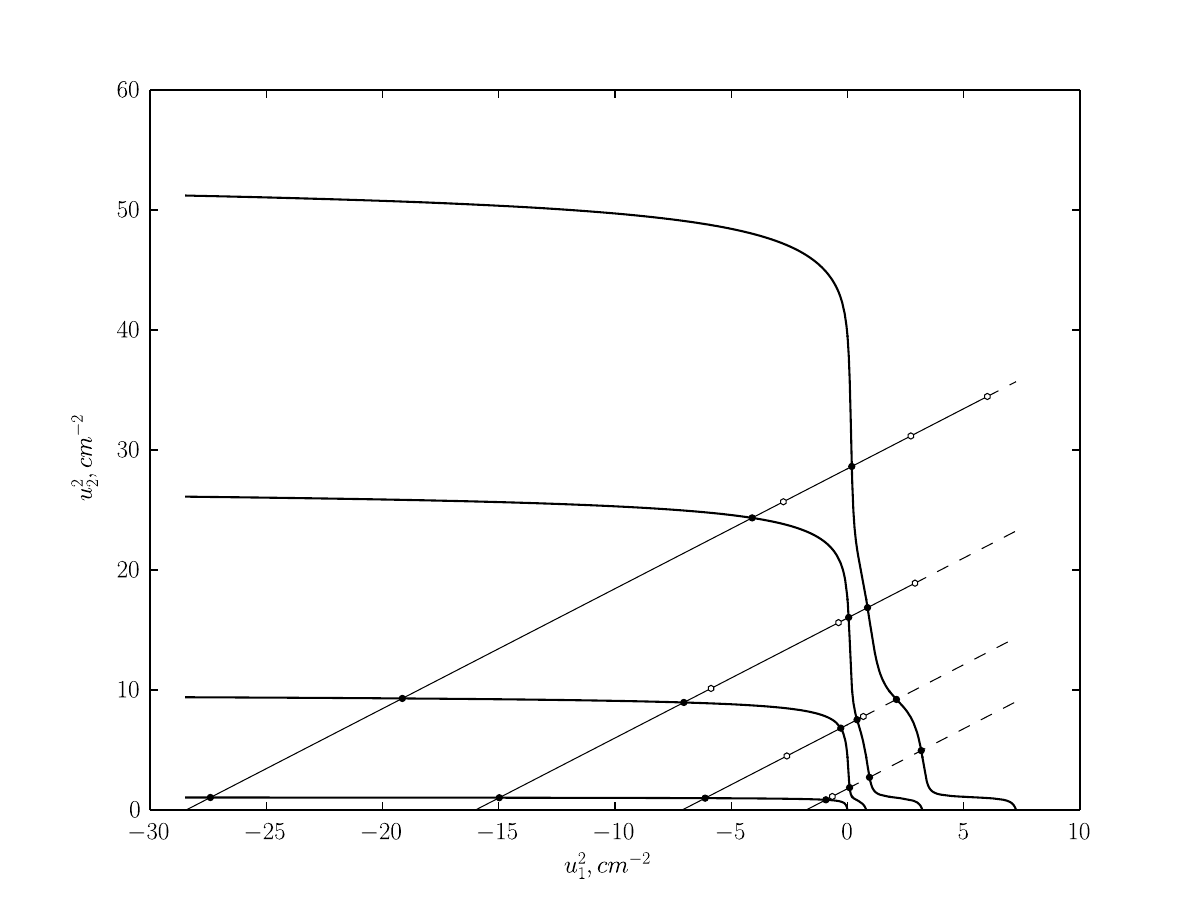
\includegraphics[width=.7\textwidth]{dispersion/lm.png}
    \caption{К определению поперечных волновых чисел для LM-волн}
    \label{fig:lm_dispersion}
\end{figure}

По известным поперечным волновым числам легко определяется продольное:
\[
    h = \sqrt{\beta_2^2 - u_2^2 - \left(\frac{\pi n}{b}\right)^2}.
\]
Таким образом, можно получить закон дисперсии \( h(\omega) \), представленный на
рисунке~\ref{fig:dispersion}. Здесь штриховой линией отмечены поверхностные
волны, а сплошной -- быстрые.

\begin{figure}[H]
    \center
    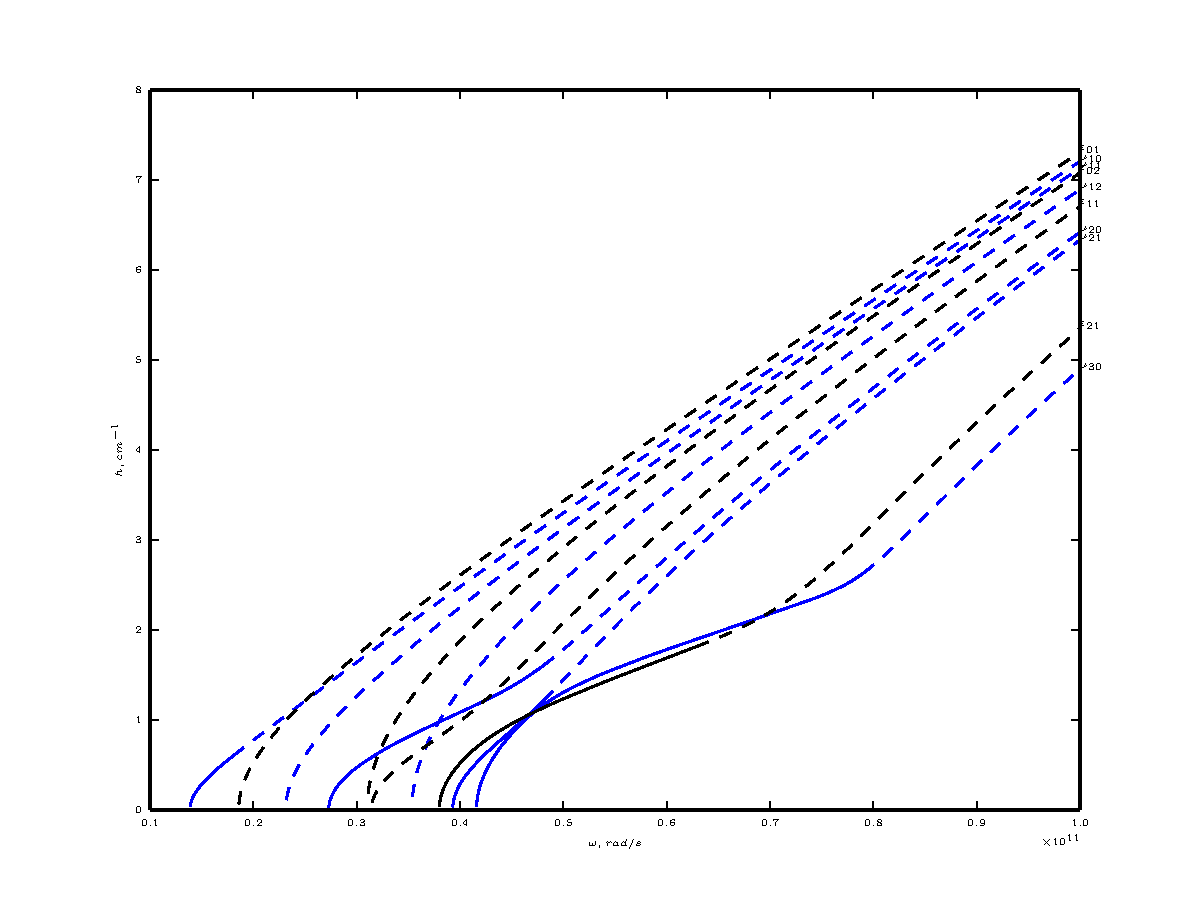
\includegraphics[width=.7\textwidth]{dispersion.pdf}
    \caption{Закон дисперсии для низших гармоник волновода}
    \label{fig:dispersion}
\end{figure}


\pagebreak
\section{Картина полей в поперечном сечении волновода}
\begin{figure}[h]
\center
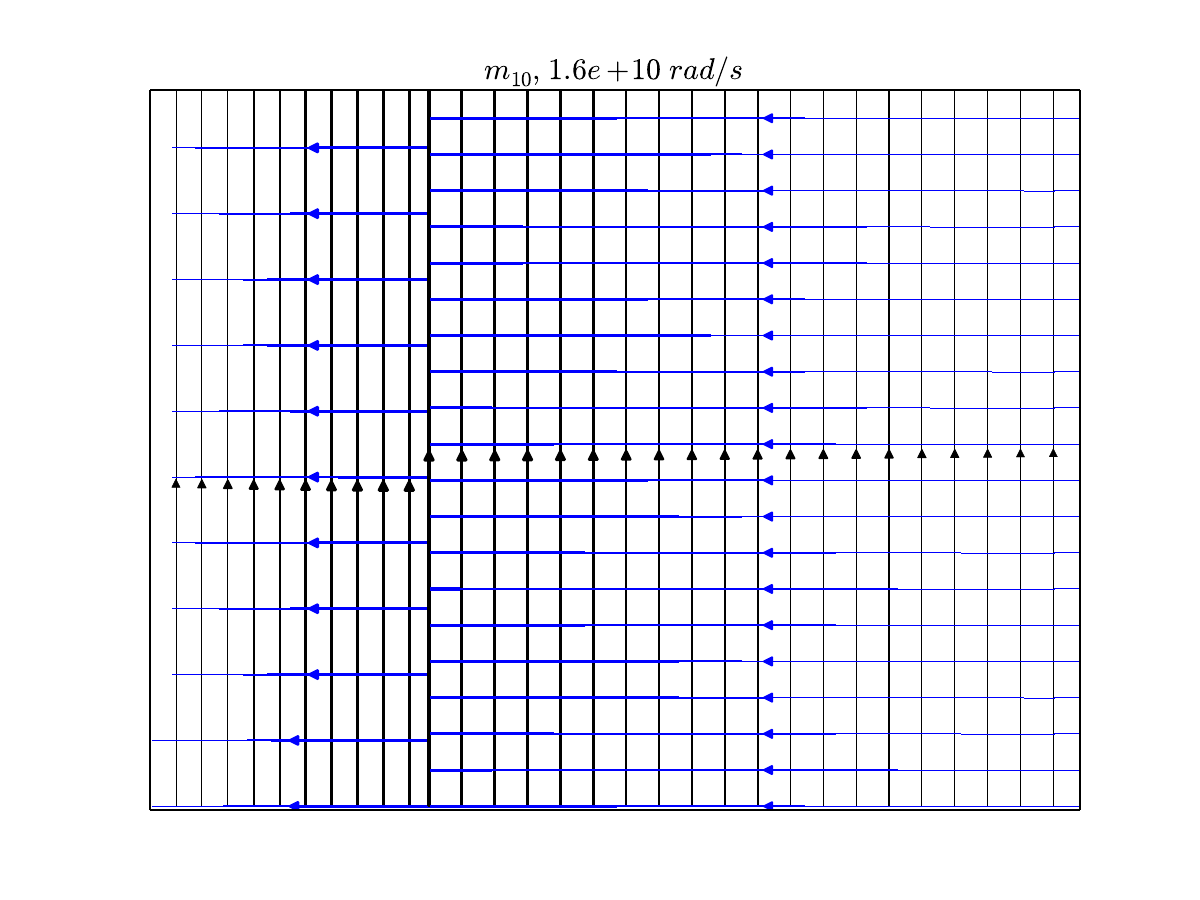
\includegraphics[width=.47\textwidth]{field/field_le_1_0_1,6e+10.png}\hfill
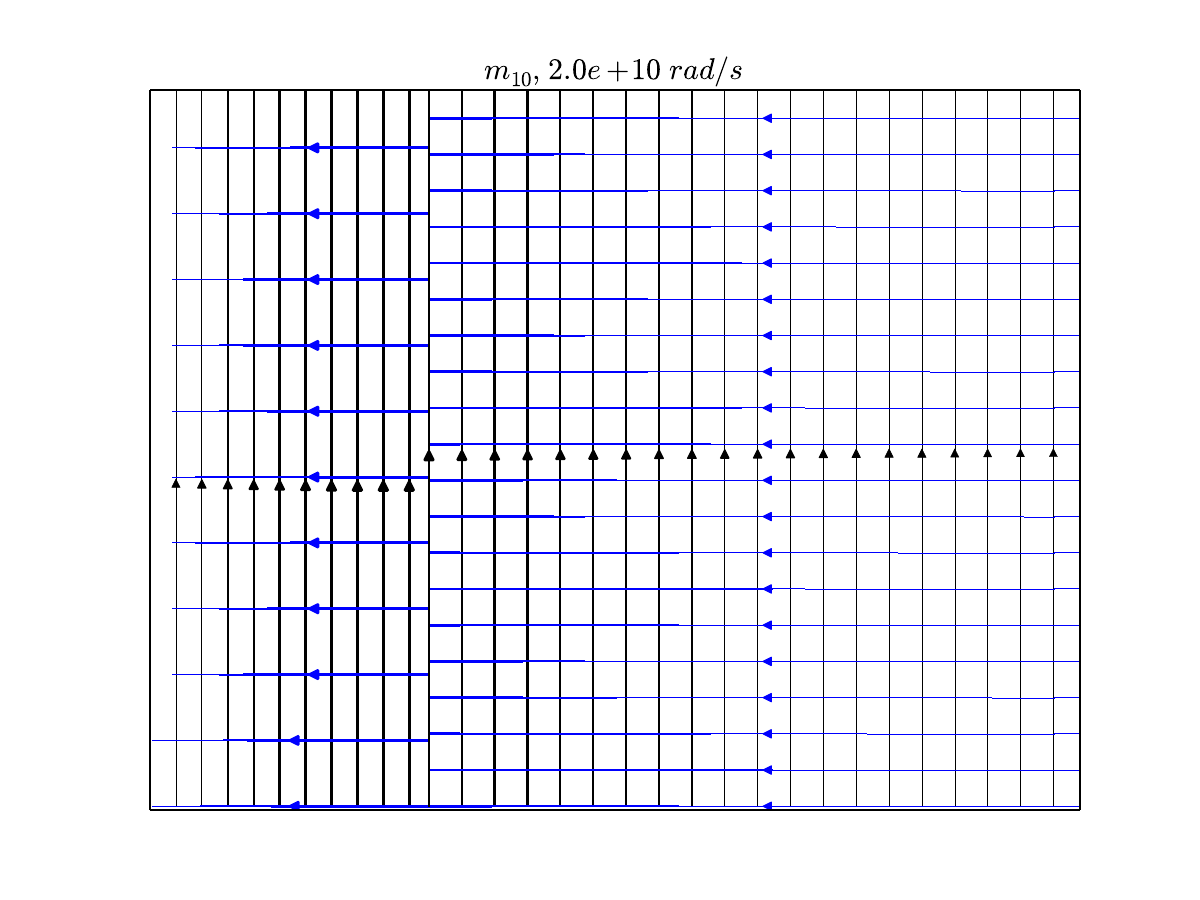
\includegraphics[width=.47\textwidth]{field/field_le_1_0_2,0e+10.png}
\caption{Волна \(LE_{10}\): быстрая \((1.6\cdot10^{10}~\text{рад/с})\) и
поверхностная \((2.0\cdot10^{10}~\text{рад/с})\)}
\end{figure}
\begin{figure}[h]
\center
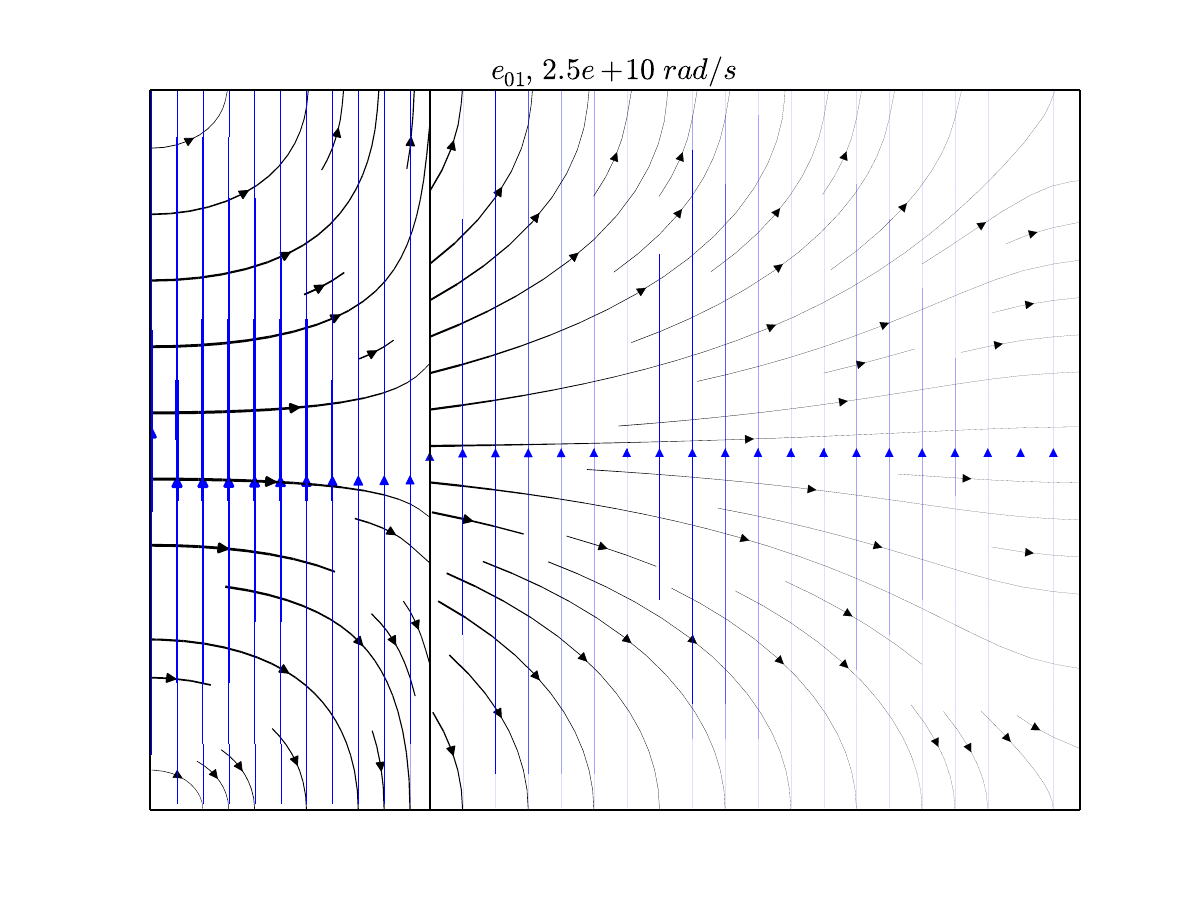
\includegraphics[width=.47\textwidth]{field/field_lm_0_1_2,5e+10.png}\hfill
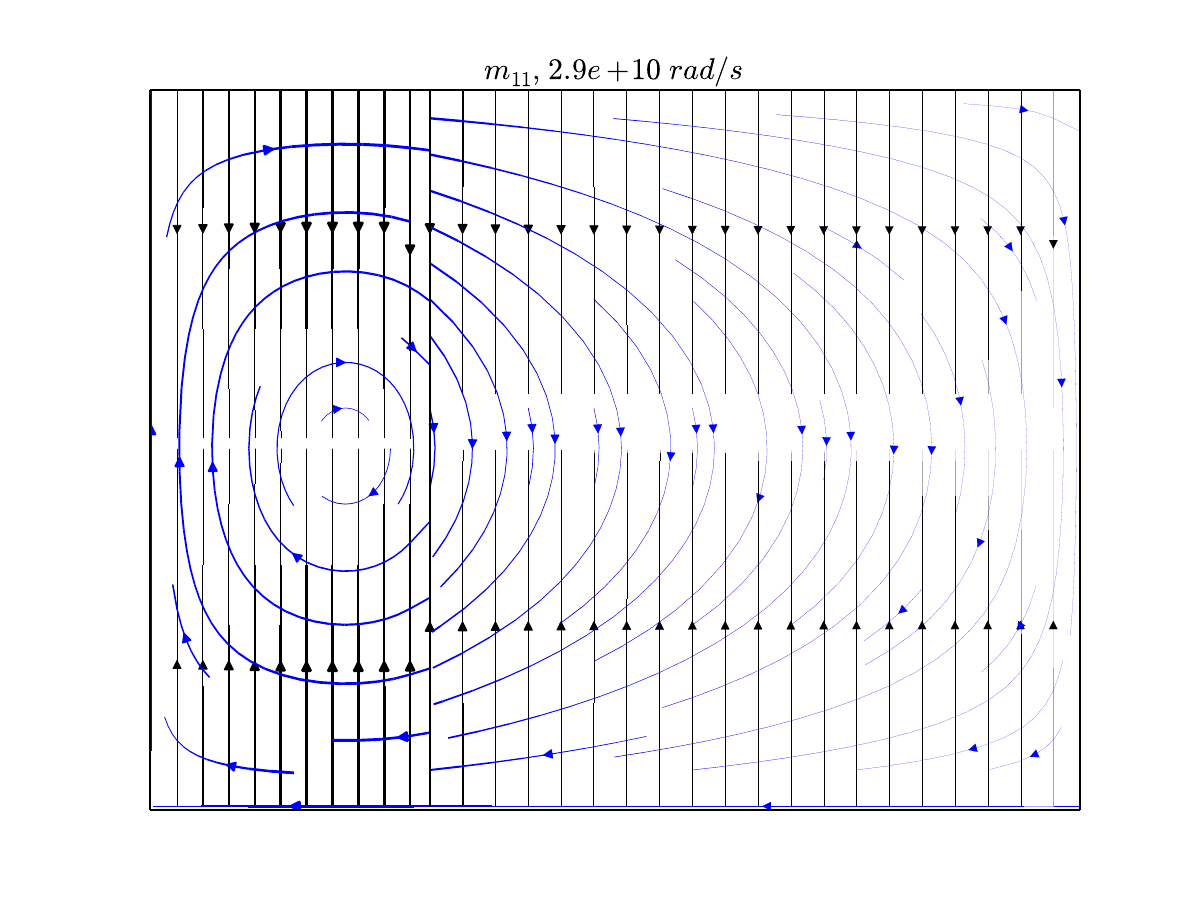
\includegraphics[width=.47\textwidth]{field/field_le_1_1_2,9e+10.png}
\caption{Волны \(LM_{01}\) и \(LE_{11}\)}
\end{figure}
\begin{figure}[h]
\center
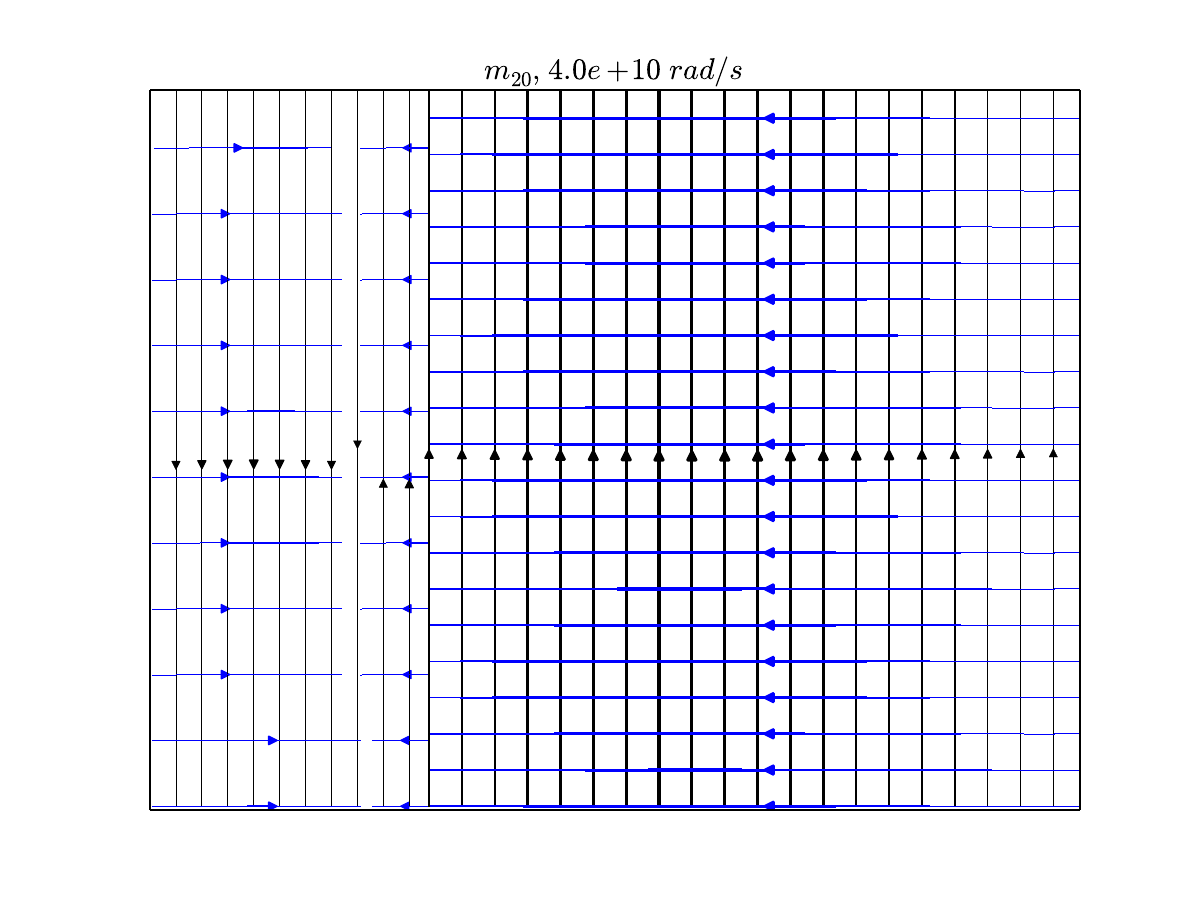
\includegraphics[width=.47\textwidth]{field/field_le_2_0_4,0e+10.png}\hfill
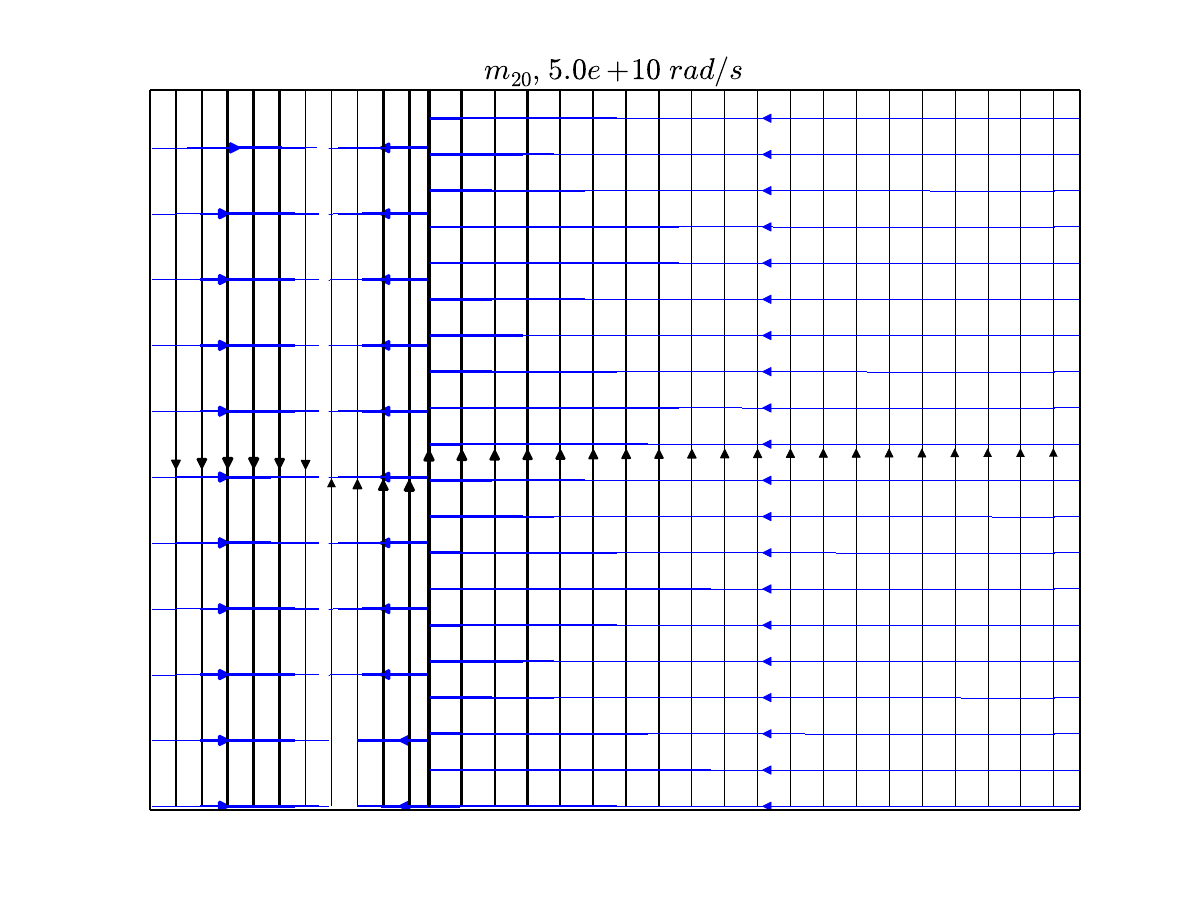
\includegraphics[width=.47\textwidth]{field/field_le_2_0_5,0e+10.png}
\caption{Волна \(LE_{20}\): быстрая \((4.0\cdot10^{10}~\text{рад/с})\) и
поверхностная \((5.0\cdot10^{10}~\text{рад/с})\)}
\end{figure}
\begin{figure}[h]
\center
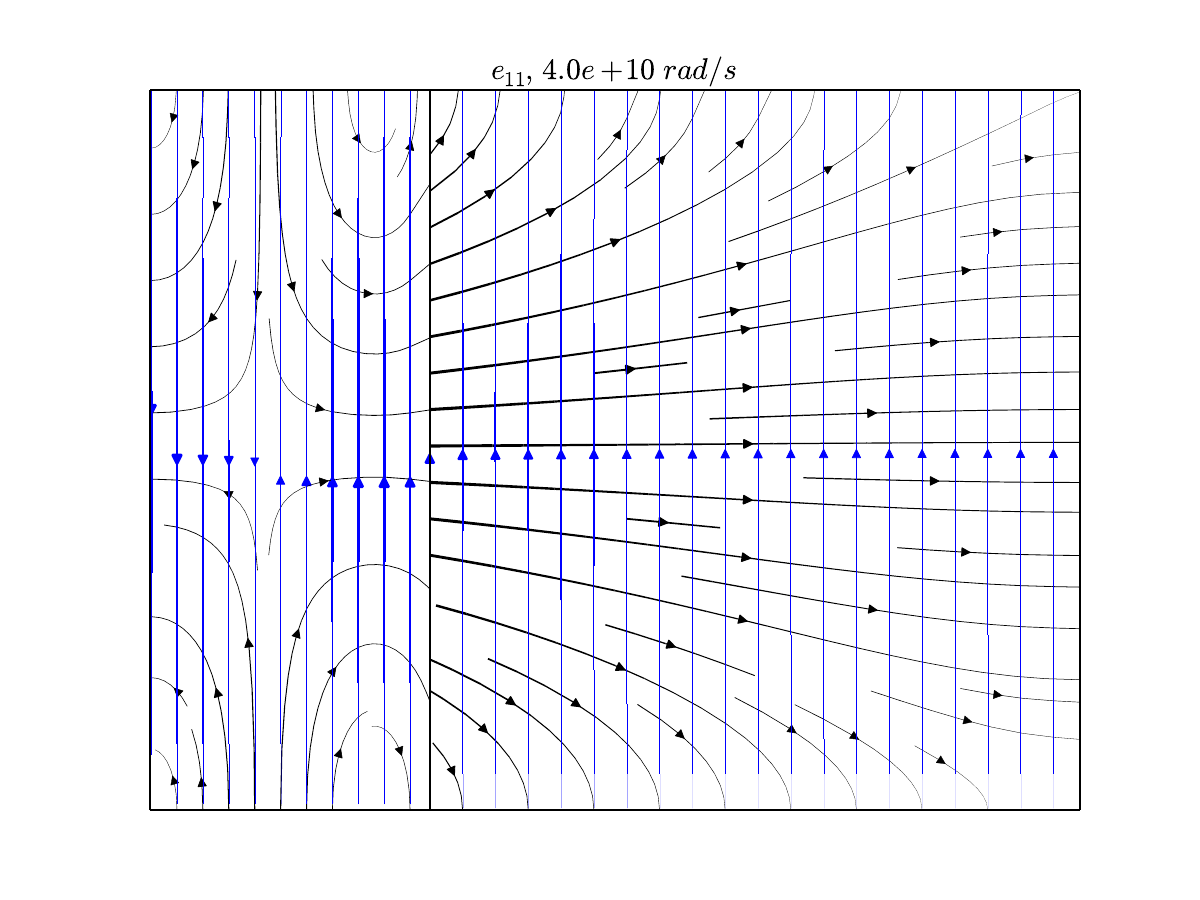
\includegraphics[width=.47\textwidth]{field/field_lm_1_1_4,0e+10.png}\hfill
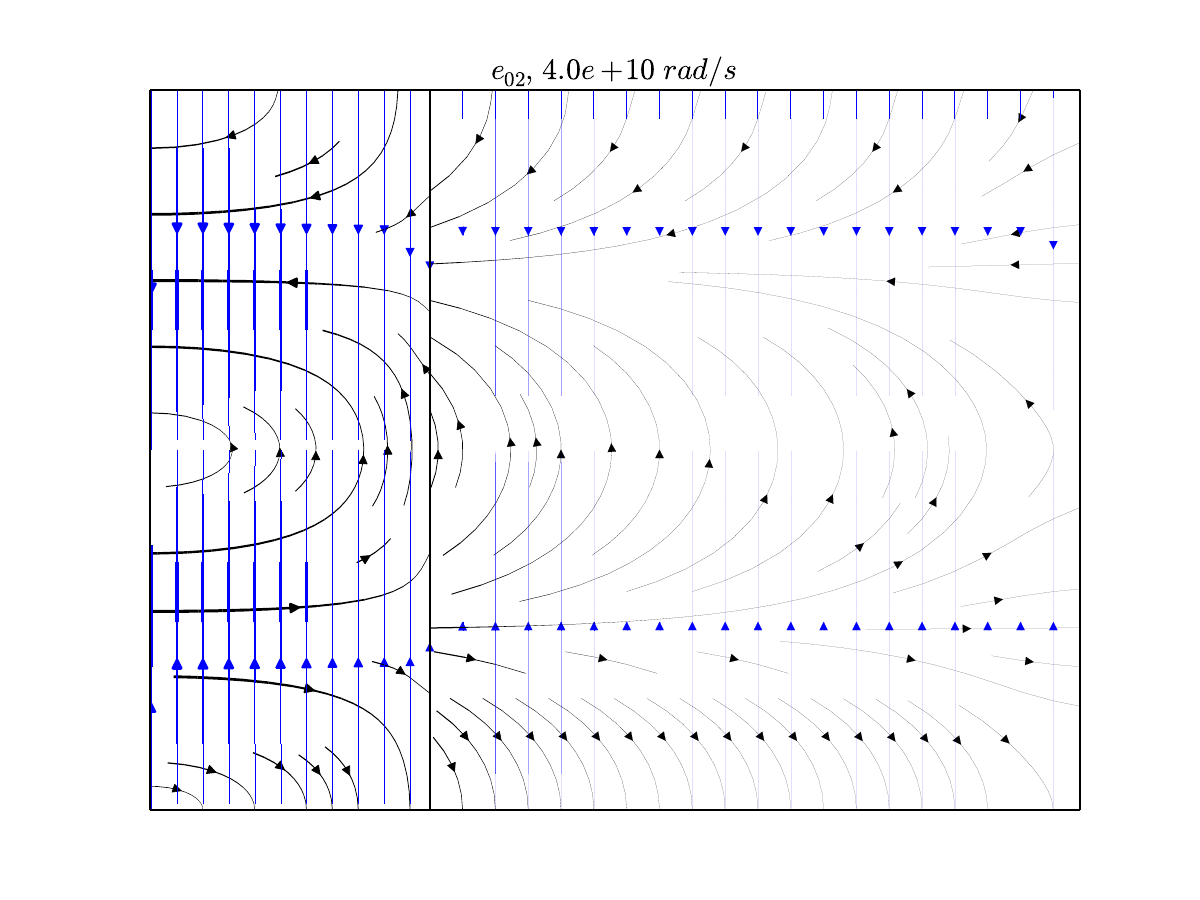
\includegraphics[width=.47\textwidth]{field/field_lm_0_2_4,0e+10.png}
\caption{Волны \(LM_{11}\) и \(LM_{02}\)}
\end{figure}
\begin{figure}[h]
\center
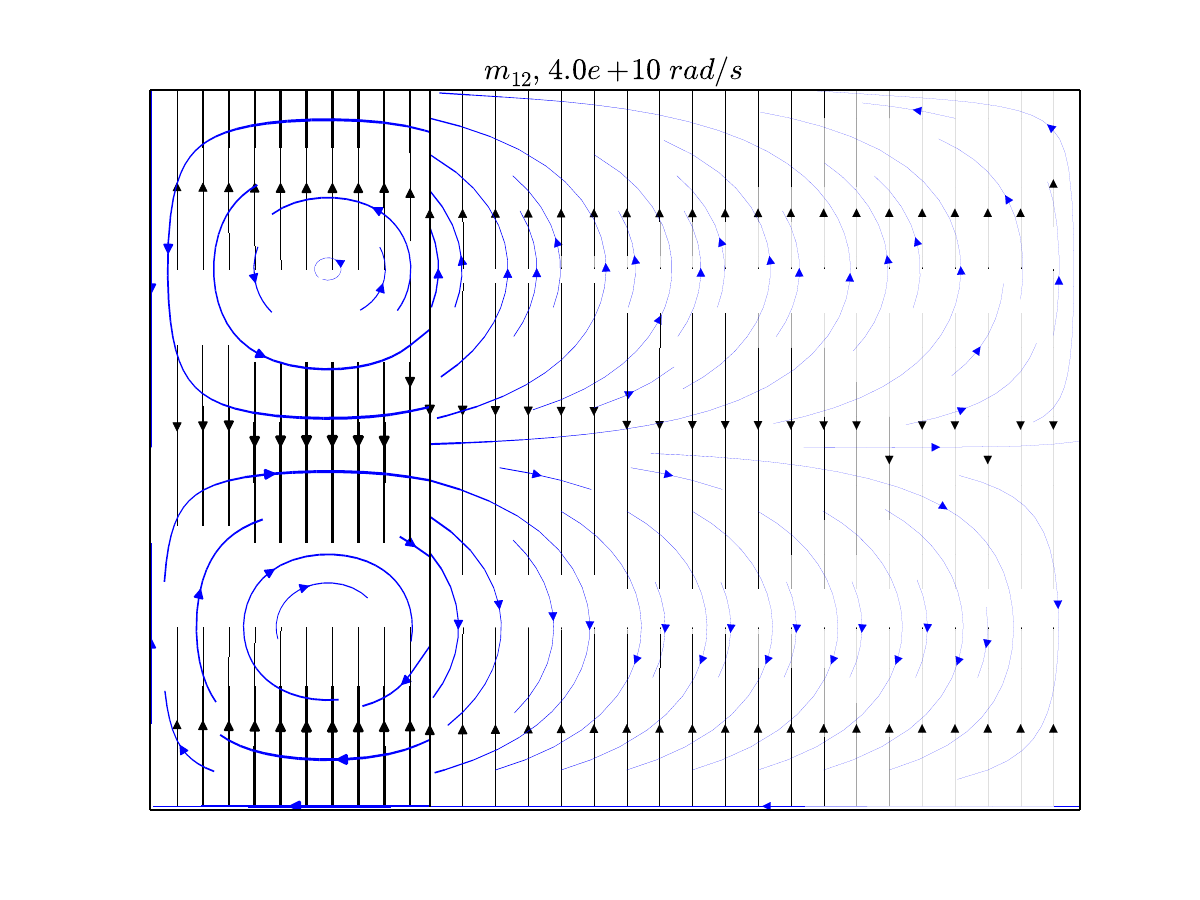
\includegraphics[width=.47\textwidth]{field/field_le_1_2_4,0e+10.png}
\caption{Волна \(LE_{12}\)}
\end{figure}
\begin{figure}[h]
\center
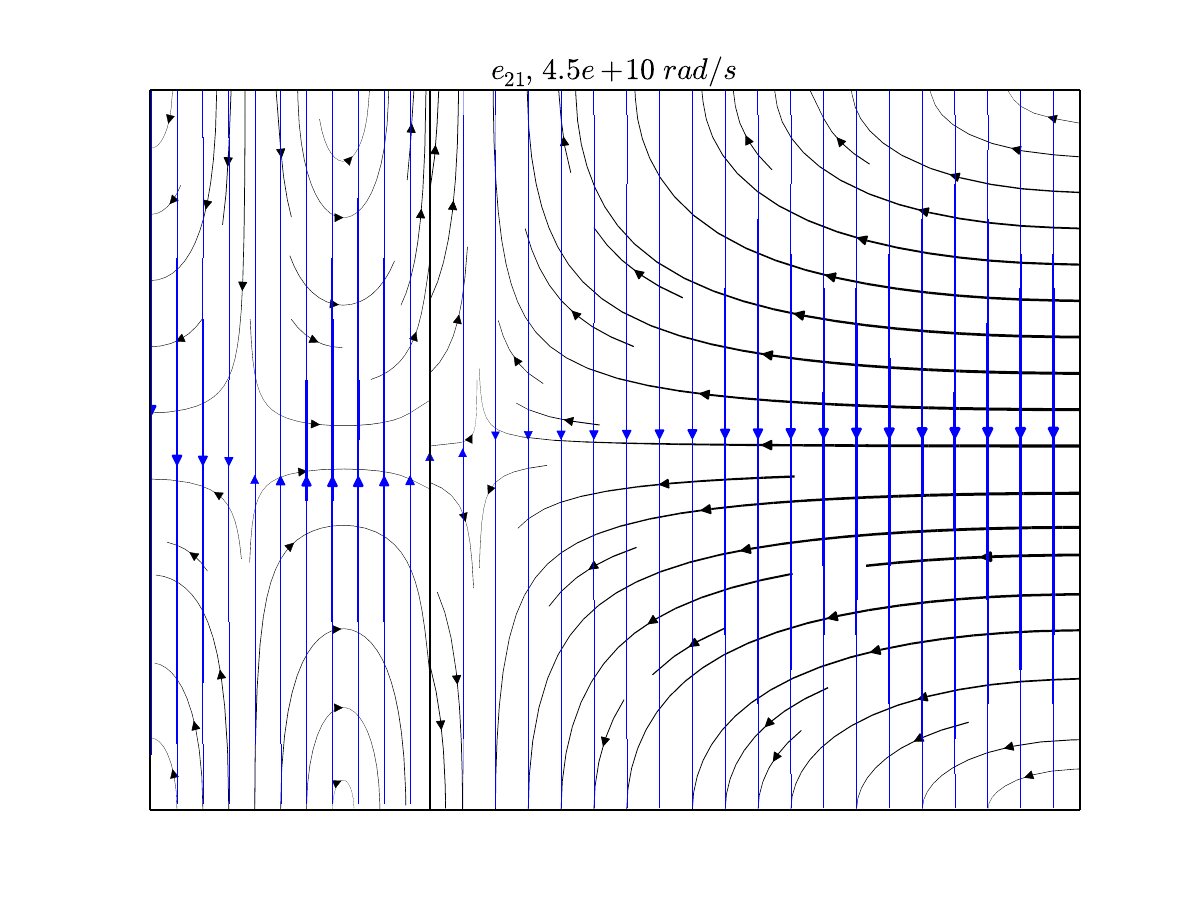
\includegraphics[width=.47\textwidth]{field/field_lm_2_1_4,5e+10.png}\hfill
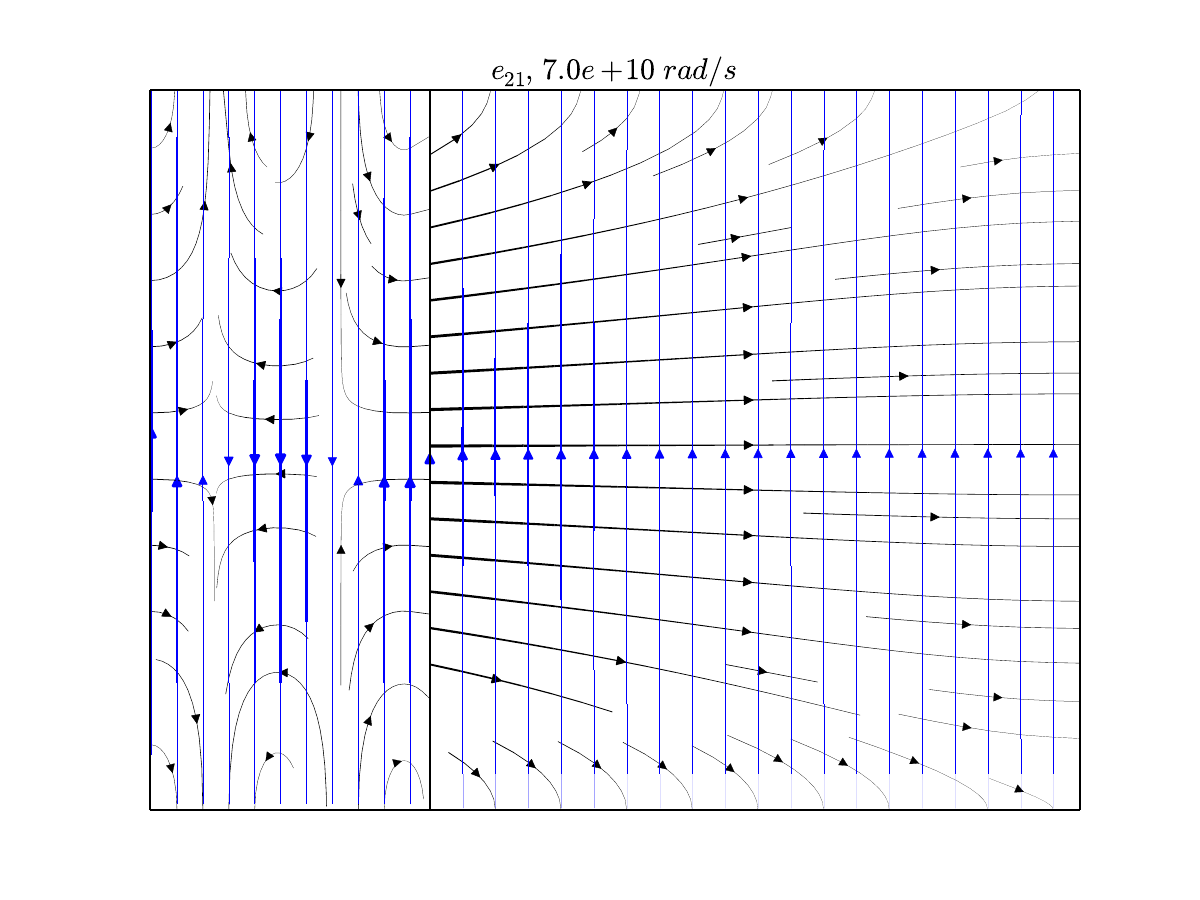
\includegraphics[width=.47\textwidth]{field/field_lm_2_1_7,0e+10.png}
\caption{Волна \(LM_{21}\): быстрая \((4.5\cdot10^{10}~\text{рад/с})\) и
поверхностная \((7.0\cdot10^{10}~\text{рад/с})\)}
\end{figure}
\begin{figure}[h]
\center
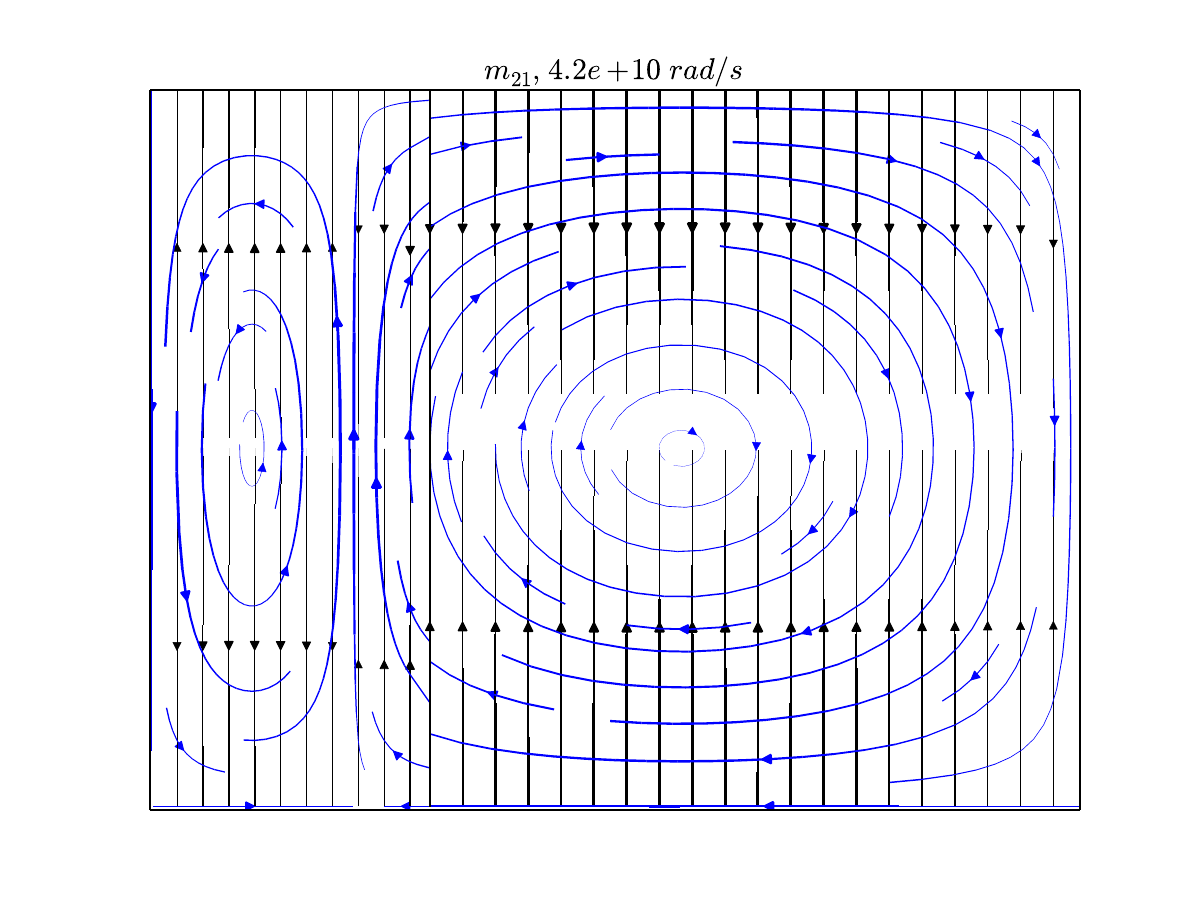
\includegraphics[width=.47\textwidth]{field/field_le_2_1_4,2e+10.png}\hfill
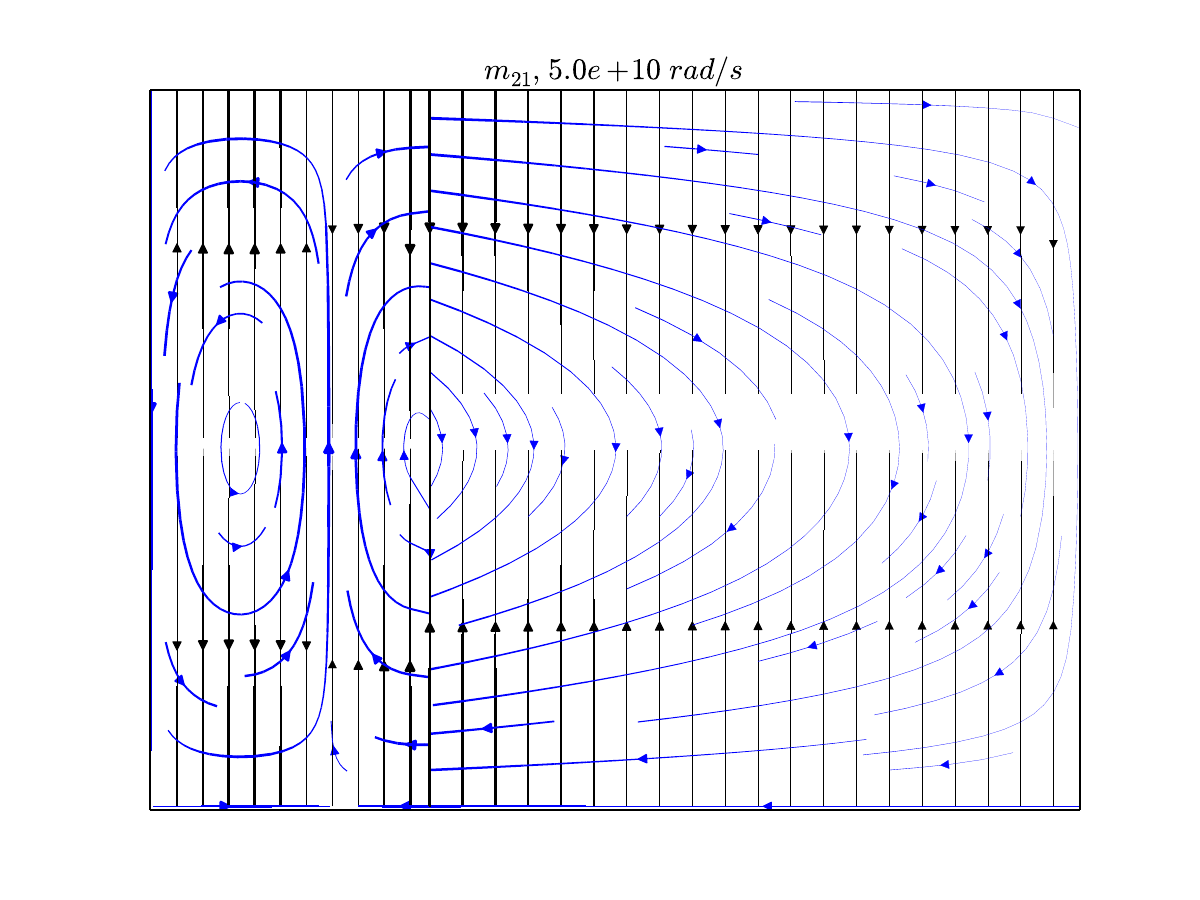
\includegraphics[width=.47\textwidth]{field/field_le_2_1_5,0e+10.png}
\caption{Волна \(LE_{21}\): быстрая \((4.2\cdot10^{10}~\text{рад/с})\) и
поверхностная \((5.0\cdot10^{10}~\text{рад/с})\)}
\end{figure}
\begin{figure}[h]
\center
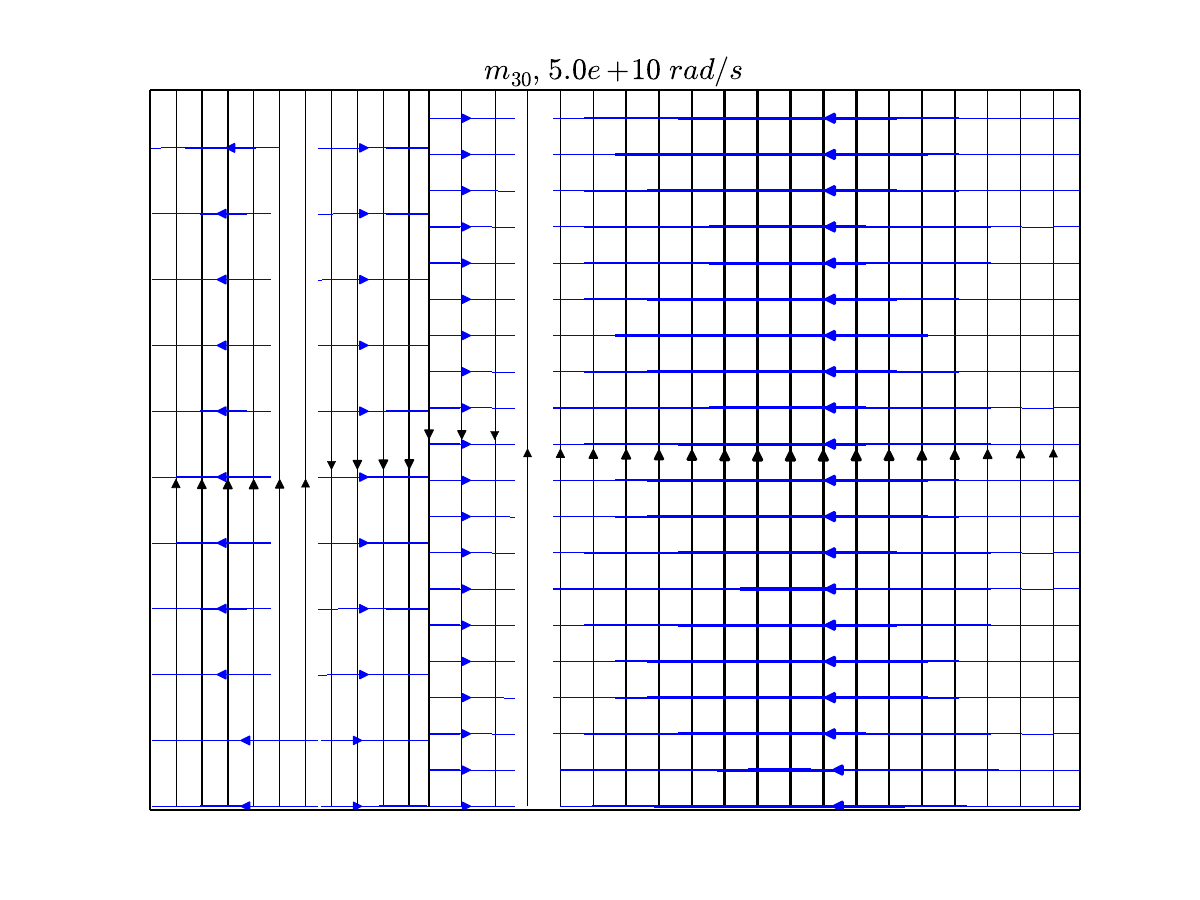
\includegraphics[width=.47\textwidth]{field/field_le_3_0_5,0e+10.png}\hfill
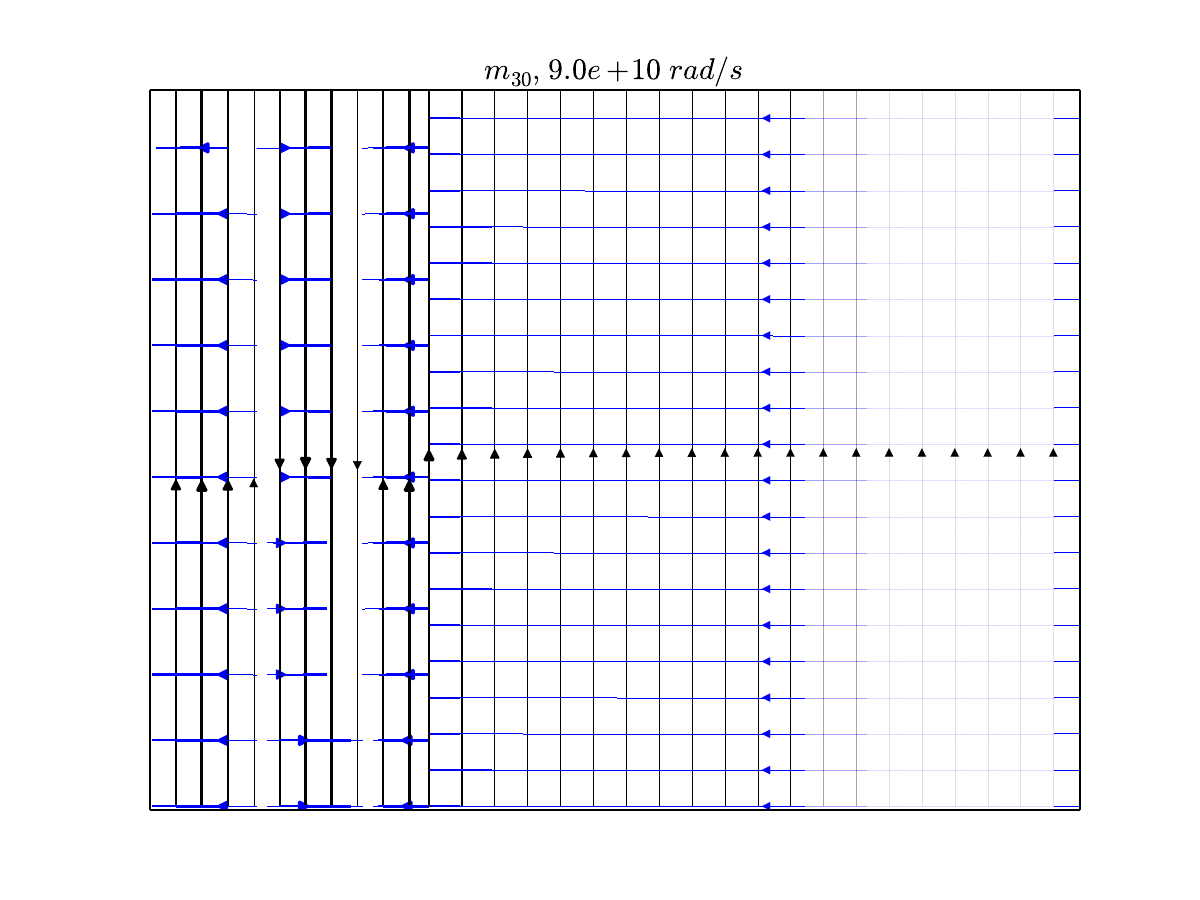
\includegraphics[width=.47\textwidth]{field/field_le_3_0_9,0e+10.png}
\caption{Волна \(LE_{30}\): быстрая \((5.0\cdot10^{10}~\text{рад/с})\) и
поверхностная \((9.0\cdot10^{10}~\text{рад/с})\)}
\end{figure}


\end{document}

